
%% bare_conf.tex
%% V1.4b
%% 2015/08/26
%% by Michael Shell
%% See:
%% http://www.michaelshell.org/
%% for current contact information.
%%
%% This is a skeleton file demonstrating the use of IEEEtran.cls
%% (requires IEEEtran.cls version 1.8b or later) with an IEEE
%% conference paper.
%%
%% Support sites:
%% http://www.michaelshell.org/tex/ieeetran/
%% http://www.ctan.org/pkg/ieeetran
%% and
%% http://www.ieee.org/

%%*************************************************************************
%% Legal Notice:
%% This code is offered as-is without any warranty either expressed or
%% implied; without even the implied warranty of MERCHANTABILITY or
%% FITNESS FOR A PARTICULAR PURPOSE! 
%% User assumes all risk.
%% In no event shall the IEEE or any contributor to this code be liable for
%% any damages or losses, including, but not limited to, incidental,
%% consequential, or any other damages, resulting from the use or misuse
%% of any information contained here.
%%
%% All comments are the opinions of their respective authors and are not
%% necessarily endorsed by the IEEE.
%%
%% This work is distributed under the LaTeX Project Public License (LPPL)
%% ( http://www.latex-project.org/ ) version 1.3, and may be freely used,
%% distributed and modified. A copy of the LPPL, version 1.3, is included
%% in the base LaTeX documentation of all distributions of LaTeX released
%% 2003/12/01 or later.
%% Retain all contribution notices and credits.
%% ** Modified files should be clearly indicated as such, including  **
%% ** renaming them and changing author support contact information. **
%%*************************************************************************


% *** Authors should verify (and, if needed, correct) their LaTeX system  ***
% *** with the testflow diagnostic prior to trusting their LaTeX platform ***
% *** with production work. The IEEE's font choices and paper sizes can   ***
% *** trigger bugs that do not appear when using other class files.       ***                          ***
% The testflow support page is at:
% http://www.michaelshell.org/tex/testflow/



\documentclass[conference]{IEEEtran}
% Some Computer Society conferences also require the compsoc mode option,
% but others use the standard conference format.
%
% If IEEEtran.cls has not been installed into the LaTeX system files,
% manually specify the path to it like:
% \documentclass[conference]{../sty/IEEEtran}

\RequirePackage[utf8]{inputenc}



% Some very useful LaTeX packages include:
% (uncomment the ones you want to load)


% *** MISC UTILITY PACKAGES ***
%
%\usepackage{ifpdf}
% Heiko Oberdiek's ifpdf.sty is very useful if you need conditional
% compilation based on whether the output is pdf or dvi.
% usage:
% \ifpdf
%   % pdf code
% \else
%   % dvi code
% \fi
% The latest version of ifpdf.sty can be obtained from:
% http://www.ctan.org/pkg/ifpdf
% Also, note that IEEEtran.cls V1.7 and later provides a builtin
% \ifCLASSINFOpdf conditional that works the same way.
% When switching from latex to pdflatex and vice-versa, the compiler may
% have to be run twice to clear warning/error messages.


% *** CITATION PACKAGES ***
\usepackage{cite}
% cite.sty was written by Donald Arseneau
% V1.6 and later of IEEEtran pre-defines the format of the cite.sty package
% \cite{} output to follow that of the IEEE. Loading the cite package will
% result in citation numbers being automatically sorted and properly
% "compressed/ranged". e.g., [1], [9], [2], [7], [5], [6] without using
% cite.sty will become [1], [2], [5]--[7], [9] using cite.sty. cite.sty's
% \cite will automatically add leading space, if needed. Use cite.sty's
% noadjust option (cite.sty V3.8 and later) if you want to turn this off
% such as if a citation ever needs to be enclosed in parenthesis.
% cite.sty is already installed on most LaTeX systems. Be sure and use
% version 5.0 (2009-03-20) and later if using hyperref.sty.
% The latest version can be obtained at:
% http://www.ctan.org/pkg/cite
% The documentation is contained in the cite.sty file itself.






% *** GRAPHICS RELATED PACKAGES ***
%
\ifCLASSINFOpdf
  \usepackage[pdftex]{graphicx}
  % declare the path(s) where your graphic files are
  % \graphicspath{{../pdf/}{../jpeg/}}
  % and their extensions so you won't have to specify these with
  % every instance of \includegraphics
  % \DeclareGraphicsExtensions{.pdf,.jpeg,.png}
\else
  % or other class option (dvipsone, dvipdf, if not using dvips). graphicx
  % will default to the driver specified in the system graphics.cfg if no
  % driver is specified.
  % \usepackage[dvips]{graphicx}
  % declare the path(s) where your graphic files are
  % \graphicspath{{../eps/}}
  % and their extensions so you won't have to specify these with
  % every instance of \includegraphics
  % \DeclareGraphicsExtensions{.eps}
\fi
% graphicx was written by David Carlisle and Sebastian Rahtz. It is
% required if you want graphics, photos, etc. graphicx.sty is already
% installed on most LaTeX systems. The latest version and documentation
% can be obtained at: 
% http://www.ctan.org/pkg/graphicx
% Another good source of documentation is "Using Imported Graphics in
% LaTeX2e" by Keith Reckdahl which can be found at:
% http://www.ctan.org/pkg/epslatex
%
% latex, and pdflatex in dvi mode, support graphics in encapsulated
% postscript (.eps) format. pdflatex in pdf mode supports graphics
% in .pdf, .jpeg, .png and .mps (metapost) formats. Users should ensure
% that all non-photo figures use a vector format (.eps, .pdf, .mps) and
% not a bitmapped formats (.jpeg, .png). The IEEE frowns on bitmapped formats
% which can result in "jaggedy"/blurry rendering of lines and letters as
% well as large increases in file sizes.
%
% You can find documentation about the pdfTeX application at:
% http://www.tug.org/applications/pdftex





% *** MATH PACKAGES ***
%
\usepackage{amsmath}
% A popular package from the American Mathematical Society that provides
% many useful and powerful commands for dealing with mathematics.
%
% Note that the amsmath package sets \interdisplaylinepenalty to 10000
% thus preventing page breaks from occurring within multiline equations. Use:
%\interdisplaylinepenalty=2500
% after loading amsmath to restore such page breaks as IEEEtran.cls normally
% does. amsmath.sty is already installed on most LaTeX systems. The latest
% version and documentation can be obtained at:
% http://www.ctan.org/pkg/amsmath





% *** SPECIALIZED LIST PACKAGES ***
%
%\usepackage{algorithmic}
% algorithmic.sty was written by Peter Williams and Rogerio Brito.
% This package provides an algorithmic environment fo describing algorithms.
% You can use the algorithmic environment in-text or within a figure
% environment to provide for a floating algorithm. Do NOT use the algorithm
% floating environment provided by algorithm.sty (by the same authors) or
% algorithm2e.sty (by Christophe Fiorio) as the IEEE does not use dedicated
% algorithm float types and packages that provide these will not provide
% correct IEEE style captions. The latest version and documentation of
% algorithmic.sty can be obtained at:
% http://www.ctan.org/pkg/algorithms
% Also of interest may be the (relatively newer and more customizable)
% algorithmicx.sty package by Szasz Janos:
% http://www.ctan.org/pkg/algorithmicx




% *** ALIGNMENT PACKAGES ***
%
\usepackage{array}
% Frank Mittelbach's and David Carlisle's array.sty patches and improves
% the standard LaTeX2e array and tabular environments to provide better
% appearance and additional user controls. As the default LaTeX2e table
% generation code is lacking to the point of almost being broken with
% respect to the quality of the end results, all users are strongly
% advised to use an enhanced (at the very least that provided by array.sty)
% set of table tools. array.sty is already installed on most systems. The
% latest version and documentation can be obtained at:
% http://www.ctan.org/pkg/array


% IEEEtran contains the IEEEeqnarray family of commands that can be used to
% generate multiline equations as well as matrices, tables, etc., of high
% quality.




% *** SUBFIGURE PACKAGES ***
%\ifCLASSOPTIONcompsoc
%  \usepackage[caption=false,font=normalsize,labelfont=sf,textfont=sf]{subfig}
%\else
  \usepackage[caption=false,font=footnotesize]{subfig}
%\fi
% subfig.sty, written by Steven Douglas Cochran, is the modern replacement
% for subfigure.sty, the latter of which is no longer maintained and is
% incompatible with some LaTeX packages including fixltx2e. However,
% subfig.sty requires and automatically loads Axel Sommerfeldt's caption.sty
% which will override IEEEtran.cls' handling of captions and this will result
% in non-IEEE style figure/table captions. To prevent this problem, be sure
% and invoke subfig.sty's "caption=false" package option (available since
% subfig.sty version 1.3, 2005/06/28) as this is will preserve IEEEtran.cls
% handling of captions.
% Note that the Computer Society format requires a larger sans serif font
% than the serif footnote size font used in traditional IEEE formatting
% and thus the need to invoke different subfig.sty package options depending
% on whether compsoc mode has been enabled.
%
% The latest version and documentation of subfig.sty can be obtained at:
% http://www.ctan.org/pkg/subfig




% *** FLOAT PACKAGES ***
%
%\usepackage{fixltx2e}
% fixltx2e, the successor to the earlier fix2col.sty, was written by
% Frank Mittelbach and David Carlisle. This package corrects a few problems
% in the LaTeX2e kernel, the most notable of which is that in current
% LaTeX2e releases, the ordering of single and double column floats is not
% guaranteed to be preserved. Thus, an unpatched LaTeX2e can allow a
% single column figure to be placed prior to an earlier double column
% figure.
% Be aware that LaTeX2e kernels dated 2015 and later have fixltx2e.sty's
% corrections already built into the system in which case a warning will
% be issued if an attempt is made to load fixltx2e.sty as it is no longer
% needed.
% The latest version and documentation can be found at:
% http://www.ctan.org/pkg/fixltx2e


\usepackage{stfloats}
% stfloats.sty was written by Sigitas Tolusis. This package gives LaTeX2e
% the ability to do double column floats at the bottom of the page as well
% as the top. (e.g., "\begin{figure*}[!b]" is not normally possible in
% LaTeX2e). It also provides a command:
%\fnbelowfloat
% to enable the placement of footnotes below bottom floats (the standard
% LaTeX2e kernel puts them above bottom floats). This is an invasive package
% which rewrites many portions of the LaTeX2e float routines. It may not work
% with other packages that modify the LaTeX2e float routines. The latest
% version and documentation can be obtained at:
% http://www.ctan.org/pkg/stfloats
% Do not use the stfloats baselinefloat ability as the IEEE does not allow
% \baselineskip to stretch. Authors submitting work to the IEEE should note
% that the IEEE rarely uses double column equations and that authors should try
% to avoid such use. Do not be tempted to use the cuted.sty or midfloat.sty
% packages (also by Sigitas Tolusis) as the IEEE does not format its papers in
% such ways.
% Do not attempt to use stfloats with fixltx2e as they are incompatible.
% Instead, use Morten Hogholm'a dblfloatfix which combines the features
% of both fixltx2e and stfloats:
%
%\usepackage{dblfloatfix}
% The latest version can be found at:
% http://www.ctan.org/pkg/dblfloatfix




% *** PDF, URL AND HYPERLINK PACKAGES ***
%
\usepackage{url}
% url.sty was written by Donald Arseneau. It provides better support for
% handling and breaking URLs. url.sty is already installed on most LaTeX
% systems. The latest version and documentation can be obtained at:
% http://www.ctan.org/pkg/url
% Basically, \url{my_url_here}.




% *** Do not adjust lengths that control margins, column widths, etc. ***
% *** Do not use packages that alter fonts (such as pslatex).         ***
% There should be no need to do such things with IEEEtran.cls V1.6 and later.
% (Unless specifically asked to do so by the journal or conference you plan
% to submit to, of course. )


% correct bad hyphenation here
\hyphenation{op-tical net-works semi-conduc-tor}


\begin{document}
%
% paper title
% Titles are generally capitalized except for words such as a, an, and, as,
% at, but, by, for, in, nor, of, on, or, the, to and up, which are usually
% not capitalized unless they are the first or last word of the title.
% Linebreaks \\ can be used within to get better formatting as desired.
% Do not put math or special symbols in the title.
\title{Classificação de Arritmias Cardíacas utilizando Transformada \textit{Wavelets} e Aprendizado de Máquina por meio de extração de características}


% author names and affiliations
% use a multiple column layout for up to three different
% affiliations
%\author{\IEEEauthorblockN{Davi Shinji Mota Kawasaki}
%\IEEEauthorblockA{Engenharia da Computa\c{c}\~ao\\
%Universidade Tecnol\'ogica Federal do Paran\'a\\
%Corn\'elio Proc\'opio/PR 86300-000\\
%Email: davishinjik@gmail.com}
%\and
%\IEEEauthorblockN{Homer Simpson}
%\IEEEauthorblockA{Twentieth Century Fox\\
%Springfield, USA\\
%Email: homer@thesimpsons.com}
%\and
%\IEEEauthorblockN{James Kirk\\ and Montgomery Scott}
%\IEEEauthorblockA{Starfleet Academy\\
%San Francisco, California 96678--2391\\
%Telephone: (800) 555--1212\\
%Fax: (888) 555--1212}}

% conference papers do not typically use \thanks and this command
% is locked out in conference mode. If really needed, such as for
% the acknowledgment of grants, issue a \IEEEoverridecommandlockouts
% after \documentclass

% for over three affiliations, or if they all won't fit within the width
% of the page, use this alternative format:
% 
\author{\IEEEauthorblockN{Davi Shinji Mota Kawasaki\IEEEauthorrefmark{1},
Higor Augusto Bassi Rozan\IEEEauthorrefmark{2},
\\João Vitor Bertoncini\IEEEauthorrefmark{3}, 
Vinícius Drago Romano\IEEEauthorrefmark{4}}
\IEEEauthorblockA{\IEEEauthorrefmark{1}Engenharia da Computação, Cornélio Procópio/PR 86300-00\\ Email: kawasaki@alunos.utfpr.edu.br}
\IEEEauthorblockA{\IEEEauthorrefmark{2}Engenharia da Computação, Cornélio Procópio/PR\\
Email: higorb.rozan@hotmail.com}
\IEEEauthorblockA{\IEEEauthorrefmark{3}Engenharia da Computação, Cornélio Procópio/PR 86300-000\\
Email: joaobertoncini@alunos.utfpr.edu.br}
\IEEEauthorblockA{\IEEEauthorrefmark{4}Engenharia da Computação, Cornélio Procópio/PR 86300-000\\ Email: romano@alunos.utfpr.edu.br}}




% use for special paper notices
%\IEEEspecialpapernotice{(Invited Paper)}




% make the title area
\maketitle

% As a general rule, do not put math, special symbols or citations
% in the abstract
\begin{abstract}
This work aims to extract and classify ventricular cardiac arrhythmias through \textit{Wavelet Transform} and machine learning algorithms. The article covers a brief theorical introduction about the medical theme, highlights the extraction window and filter methods, and then train the extracted data through a machine learning software. After that's all covered, it shows the analysis of results with two different types of machine learning algorithms with \textit{WEKA} software.
\end{abstract}

Keywords - Arrhythmias, Feature Extraction, Wavelet Transform, Neural Network, Machine Learning, WEKA, MATLAB.


% For peer review papers, you can put extra information on the cover
% page as needed:
% \ifCLASSOPTIONpeerreview
% \begin{center} \bfseries EDICS Category: 3-BBND \end{center}
% \fi
%
% For peerreview papers, this IEEEtran command inserts a page break and
% creates the second title. It will be ignored for other modes.
\IEEEpeerreviewmaketitle



\section{Introdução}
% no \IEEEPARstart

O ser humano, desde as épocas antigas, tem passado por inúmeras evoluções, assim como também por vários obstáculos pessoais, biológicos e sociais. Os contextos históricos detalham com maestria cada ponto focal característico dentre a história humana milenar, seja pelas conquistas, descobertas, guerras, expansões populacionais e, principalmente, as evoluções e revoluções marcantes.

Nesses contextos sociais, uma \textit{"persona"} sempre esteve presente dentre os momentos históricos humanos, marcando presença principalmente em fatos históricos globais. As enfermidades e doenças produziram significados que iam além das características biológicas - como foi o caso da peste negra -, demonstrando que, além de soluções médicas-científicas, eram necessários investigações socioculturais \cite{barata06}.

Com estimativas da Organização das Nações Unidas (ONU) de que a Terra terá pouco mais de 9 bilhões de habitantes em 2050, a preocupação com enfermidades tem se tornado um tópico cada vez mais alarmante globalmente. De acordo com pesquisas da FAO 1999 e UNICEF 2002, cerca de 18 milhões de seres humanos têm morrido precocemente de doenças curáveis - equivalente a possíveis 50 mil mortes que poderiam ser evitadas diariamente. Além disso, problemas médicos que causam essas doenças aplicam uma grande tensão econômica principalmente em países subdesenvolvidos, intensificando a pobreza e o nível da população doente \cite{pogge05}.

Entre essas várias doenças, as ocasionadas por insuficiências cardíacas e/ou infartos são razões da morte de aproximadamente 17,5 milhões de pessoas por ano no mundo \cite{whf02}. Segundo a Federação Mundial do Coração (FMC) esses dados demonstram que infartos derivados de problemas cardíacos são uma das principais causas de mortalidade no mundo. A ONG FMC destacou que 80\% dessas mortes ocorrem em países com nível de renda médio e baixo \cite{whf02}, caso do Brasil.

O número de infartos e doenças cardíacas vem aumentando devido a alguns fatores gerais, como o sedentarismo, má qualidade da alimentação, estresse, além de outros problemas comuns na cultura de um mundo capitalista globalizado \cite{beckert09}.

Para reduzir a quantidade de óbitos consequentes de doenças, profissionais da área da saúde têm investido em ferramentas que possam completar os diagnósticos - sejam de prevenção ou até mesmo emergenciais. Essa antecipação de descoberta de alguma doença - como disfunções cardíacas - podem determinar tratamentos médicos e até mesmo evitar mortes súbitas de pacientes.

Com o crescimento do número de pacientes dentre a volumosa população mundial, cada vez mais métodos automáticos de diagnósticos são necessários para auxiliar os médicos. Um dos caminhos para este diagnóstico, no caso de exames cardiológicos, consiste na utilização do sinal de eletrocardiograma (ECG). A alteração e distúrbios das ondas do ECG podem indicar alterações do ritmo cardíaco, também denominadas como arritmias cardíacas \cite{beckert09}, objetivo principal de análise desse artigo. Essas alterações do ritmo cardíaco normalmente são coletadas de forma analógica, ou seja, por análise gráfica visual por profissionais especialistas, o que torna a tarefa extremamente manual e não replicável.

Sob essa análise contextual, esse trabalho propõe formular um algoritmo que seja capaz de detectar, analisar e classificar automaticamente essas arritmias cardíacas. Conforme a análise literária \cite{beckert09}, algoritmos que realizam esse trabalho dificilmente alcançam taxas de 100\% de acerto. Para ultrapassar essa barreira, um método será desenvolvido para analisar o sinal de ECG, extrair características relevantes do mesmo e, por fim, classificar cada um dos sinais por dois tipos de Aprendizado de Máquina: Redes Neurais e Árvores de Decisão. Os sinais serão obtidos diretamente da base de dados \textit{MIT-BIH} - \textit{Arrhythmia Database}, e o foco de classificação dessa base serão sinais de ECG normais ou possuidor de um dos três tipos de arritmias ventriculares: Taquicardia Ventricular (VT), Bigeminismo Ventricular (B) e Trigeminismo Ventricular (T).

Por meio da normalização e filtro dos sinais, pretende-se avaliar os resultados através da taxa de acurácia do aprendizado de máquina com o \textit{software} WEKA, além de analisar a contribuição da extração dos resultados no resultado do aprendizado de máquina. 

O trabalho, portanto, é dividido em: Introdução, Fundamentação Teórica, Metodologia, Extração de Características, Treinamento com Aprendizado de Máquina, Resultados e Discussões, Conclusão.

%\hfill mds
 
%\hfill August 26, 2015

\section{Fundamentação Teórica}

\subsection{Coração}

O coração consiste em um órgão localizado atrás da caixa toráxica, na parte central do peito entre o pulmão direito e esquerdo \cite{nih11}. Sua função consiste no batimento ou contração para bombeamento do sangue para todo o corpo por meio de um sistema de vasos sanguíneos \cite{gray79}.

Para realizar o processo de bombeamento de sangue, o coração depende da sua seção direita e esquerda, onde cada uma delas possui duas cavidades: átrio e ventrículo, sendo a primeira superior e a segunda inferior. O fluxo do sangue é realizado por meio de válvulas entre o átrio e o ventrículo, sempre seguindo a direção do primeiro para o segundo.

Por meio dessas válvulas é possível realizar o processamento do oxigênio e do gás carbônico, onde a seção esquerda do coração é responsável pelo envio de sangue com oxigênio para o corpo, enquanto a direita cuida do recebimento do sangue com gás carbônico de diferentes partes do corpo \cite{nih11}. A cada contração de cada câmara do miocárdio - fluxo de sangue entre o átrio e o ventrículo - acontece o evento chamado de sístole, enquanto no relaxamento ocorre a diástole - processo o qual é repassado para o pulmão para realização da troca de gases \cite{nih11}.

\begin{figure}[!h]
	\centering
	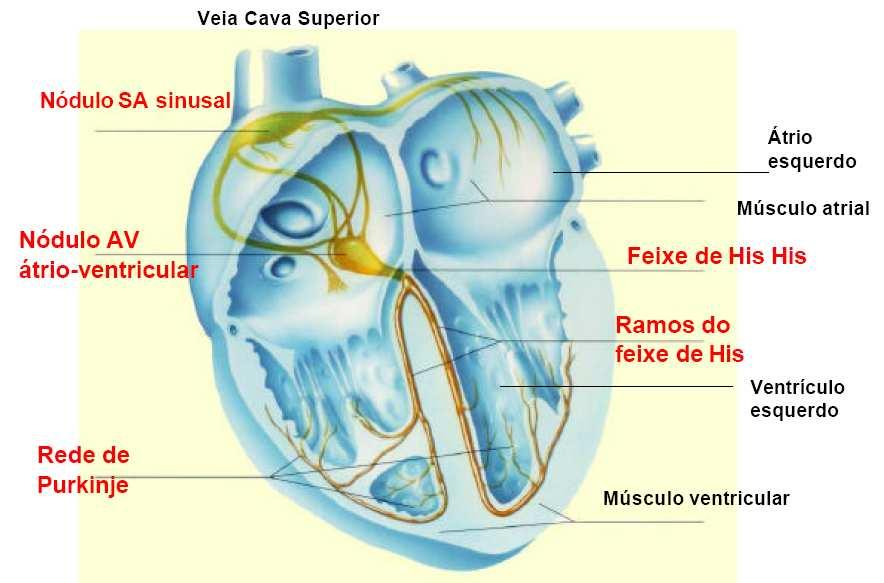
\includegraphics[width=3in]{img/coracaoEsquematico}
	\caption{Representação interna do coração e suas cavidades.}
	\label{coracaoEsquematico}
\end{figure}

Uma das estruturas internas primordiais para determinar o ritmo do coração chama-se nódulo sinoatrial (SA), ou também chamado de marca-passo. Localizada entre o átrio direito e a veia cava superior (vide Figura \ref{coracaoEsquematico}), ele atua controlando a frequência dos batimentos cardíacos, com cerca de 72 contrações por minuto. Por ter uma frequência alta, seus impulsos se espalham para os átrios e ventrículos, excitando todas as áreas e determinando o ritmo de batimento de quase todo o coração  \cite{guyton06}.

O coração, por meio do seu batimento, realiza vários eventos cardíacos chamados de ciclos cardíacos, começando pela geração de um potencial de ação propagado pelos átrios até chegar nos ventrículos. Esse ciclo cardíaco vai conter o relaxamento pela diástole (coração enche de sangue) e a sístole (contração das câmaras de bombeamento). Conforme representado pelos traçados da Figura \ref{eventosCicloCardiaco}, pode-se visualizar os períodos de pressão (mm Hg), volume (ml), eletrocardiograma e fonocardiograma, sendo o penúltimo a representação gráfica utilizada nesse trabalho para classificação de arritmias.

\begin{figure}[!h]
	\centering
	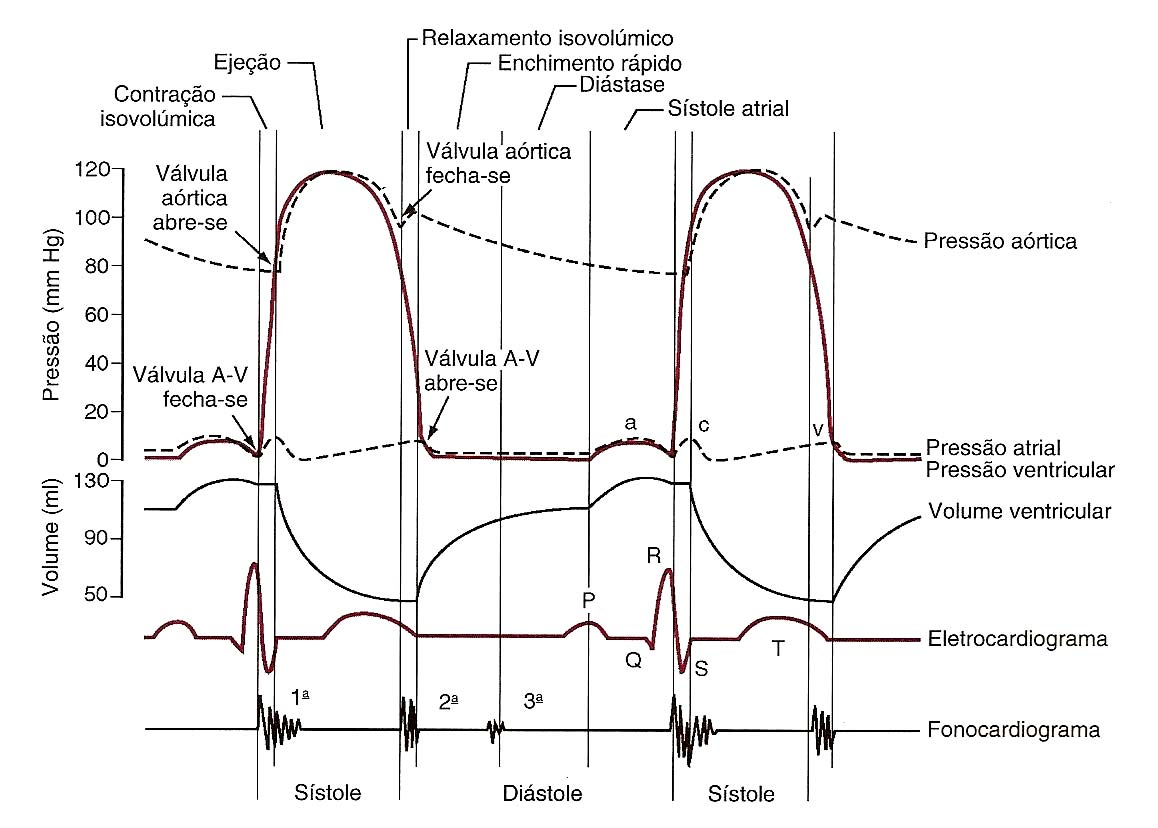
\includegraphics[width=3in]{img/eventosCicloCardiaco}
	\caption{Eventos do ciclo cardíaco representados por diferentes traçados no ventrículo esquerdo.}
	\label{eventosCicloCardiaco}
\end{figure}

\subsection{Eletrocardiograma (ECG)}

Conforme visualizado no tópico anterior, o nódulo sinoatrial (SA) determina o ritmo do coração por seus impulsos com uma frequência alta. A partir dessa excitação, ocorre paralelamente a propagação de correntes do campo elétrico no músculo cardíaco e nos tecidos das regiões vizinhas, inclusive atingindo a superfície do corpo. Como esse fluxo ocorre entre diversos locais do corpo, pode-se captar diferenças de potenciais por meio de eletrodos na pele, em pontos opostos do coração. Essas medidas podem ser coletadas por meio de 12 derivações clássicas, normalmente se baseando pelo triângulo de Einthoven, representado pela Figura \ref{trianguloEinthoven}.

\begin{figure}[!h]
	\centering
	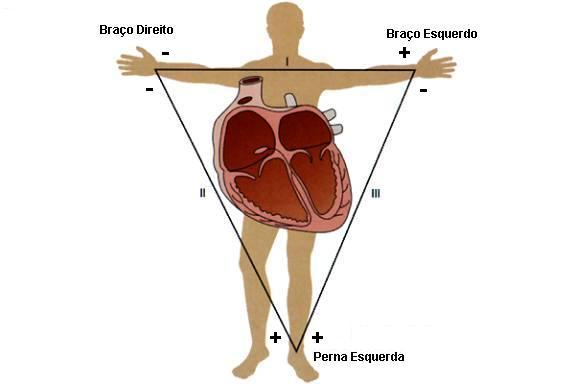
\includegraphics[width=3in]{img/trianguloEinthoven}
	\caption{Representação do triângulo de Einthoven, com eletrodos sobre os pulsos (RA e LA) e no tornozelo esquerdo (LL).}
	\label{trianguloEinthoven}
\end{figure}

Por meio de um amplificador, esses potenciais são adquiridos por um período de tempo, em localizações conforme estabelecidas pelas derivações. Esse processo trata-se da eletrocardiografia, também conhecida como o exame de eletrocardiograma (ECG), apresentando a excitação cardíaca de forma gráfica para análise patológica por um cardiologista. Esse exame de baixo custo permite a análise de uma cardiopatia/arritmia no momento de ocorrência da mesma, analisando normalmente os segmentos, intervalos e ondas do sinal de ECG.

Um registro de ECG, representado na Figura \ref{eletrocardiogramaIntervalos}, é representado por meio da voltagem plotada no eixo y pelo tempo no eixo x, onde seu sinal traduz o registro das despolarizações e repolarizações por meio de cinco etapas, representadas pelos formatos de onda P, Q, R, S e T \cite{mello91}.

\begin{figure}[!h]
	\centering
	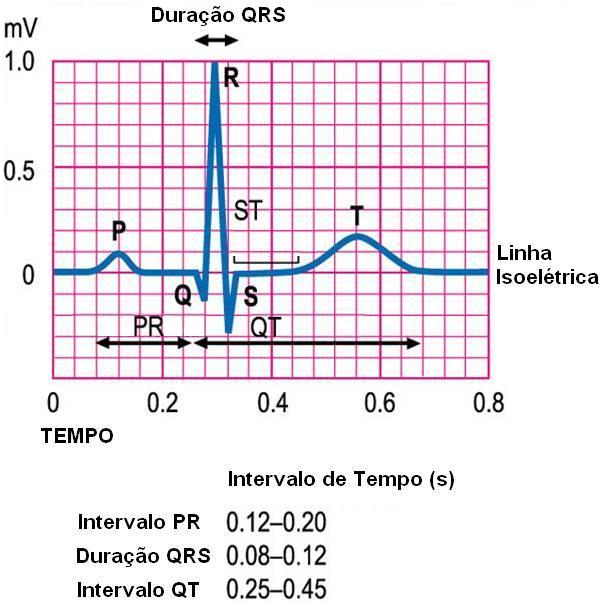
\includegraphics[width=3in]{img/eletrocardiogramaIntervalos}
	\caption{Registro de eletrocardiograma com diferentes tipos de intervalos.}
	\label{eletrocardiogramaIntervalos}
\end{figure}

Além dos formatos de onda, o ECG apresenta alguns subperíodos que são importantes para uma análise mais detalhada das cardiopatias, como o intervalo entre a onda P e R, o qual representa o tempo de condução do estímulo através do nódulo atrioventricular; e o complexo QRS, que representa a despolarização ventricular. A partir desses subperíodos pode-se analisar as morfologias do exame, denominadas pela sequência de excitação e recuperação, respectivamente caracterizados pela despolarização e repolarização por meio da
diferença de potencial resultante, conforme representado pela Figura \ref{sequenciaDespolarizacacoPolarizacao}.

\begin{figure}[!h]
	\centering
	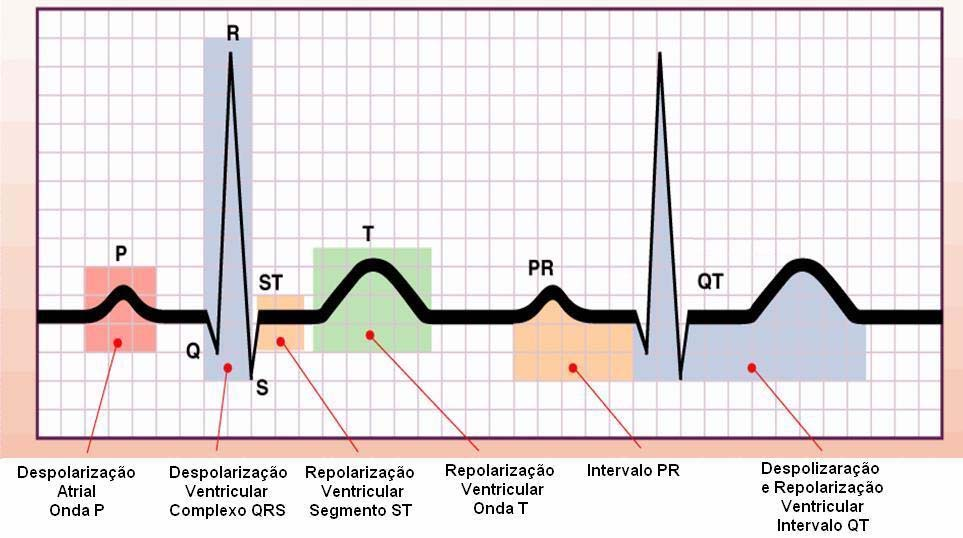
\includegraphics[width=3in]{img/sequenciaDespolarizacacoPolarizacao}
	\caption{Sequência de despolarização e repolarização com a representação das ondas e subperíodos.}
	\label{sequenciaDespolarizacacoPolarizacao}
\end{figure}

Estas morfologias permitem a verificação de anormalidades no sistema de condução cardíaca, como as arritmias que vão ser classificadas por meio de aprendizado de máquina nesse trabalho.

\subsection{Arritmias}

Conforme apresentado, os exames de ECG permitem identificar anormalidades no sistema cardiológico, podendo representar diferentes cardiopatias. Elas podem ser sintomaticamente representadas por arritmias cardíacas, que ocorrem por alterações na formação/condução do impulso elétrico através do miocárdio \cite{sbc03}. O ECG é um dos principais exames para estudo e análise das arritmias, justamente porque as mesmas podem modificar a origem/difusão fisiológica do estímulo elétrico, alterando o ritmo cardíaco normal \cite{goncalves95}.

Dentre os mais diversos tipos de classificação de arritmias, elas podem ser divididas em duas categorias (assintomáticas e sintomáticas) e em dois grupos de frequência: bradicardia - frequência cardíaca menor que 60 batimentos por segundo, e taquicardia - frequência cardíaca maior que 100 batimentos por segundo \cite{guyton06}.

O enfoque desse trabalho reside nas arritmias que ocorrem na parte ventricular do batimento cardíaco, como as seguintes: Taquicardia Ventricular (VT), Bigeminismo Ventricular (B) e Trigeminismo Ventricular (T).

A taquicardia acontece quando a frequência cardíaca é maior que 100 batimentos por minuto. Ao realizar esforços físicos sua ocorrência é considerada normal, porém após alguns minutos depois do término da atividade física, a frequência cardíaca deve se restabelecer ao nível saudável \cite{beckert09}. Quando isso não acontece ou se em repouso apresenta-se taquicardia, isto pode indicar a existência de alguma patologia, como a taquicardia ventricular representada pela Figura \ref{ecgTaquicardiaVentricular}.

\begin{figure}[!h]
	\centering
	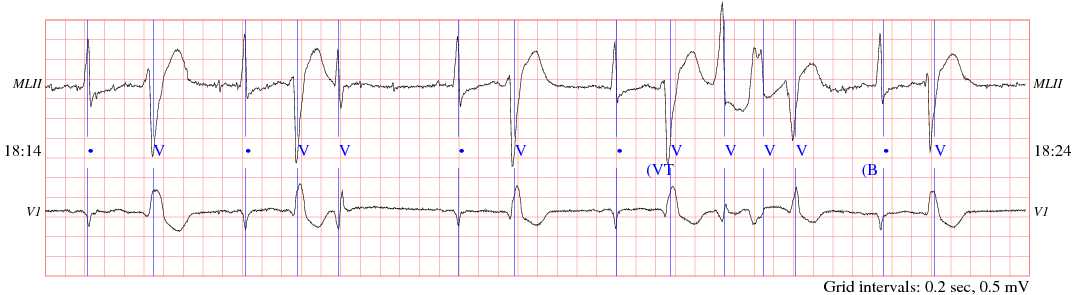
\includegraphics[width=3in]{img/ecgTaquicardiaVentricular}
	\caption{Exemplo de ECG com Taquicardia Ventricular.}
	\label{ecgTaquicardiaVentricular}
\end{figure}

Já os casos de Bigeminismo e Trigeminismo ocorrem por contrações ventriculares prematuras (PVC), onde cada PVC é seguido por uma pausa compensatória que permite que o nódulo sinoatrial descanse no ciclo, conforme representado na Figura \ref{arritmiaBigeminismoTrigeminismo}. Enquanto no bigeminismo um PVC ocorre em todas as outras batidas de forma constante, o trigeminismo consiste em um PVC ocorrendo somente na terceira batida, onde aparece uma pausa compensatória após essa batida \cite{wanderer09}.

\begin{figure}[!h]
	\centering
	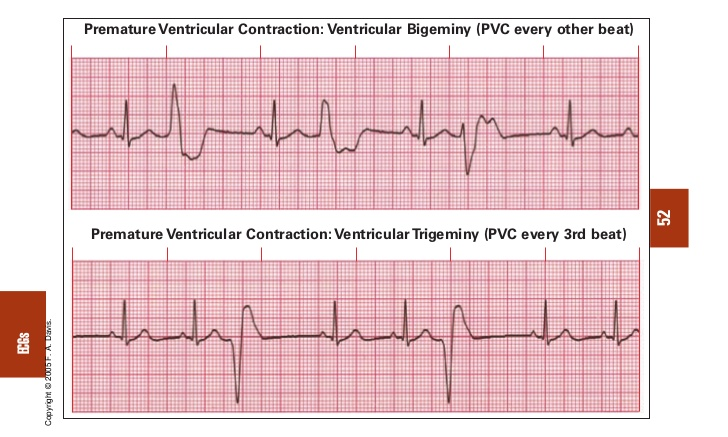
\includegraphics[width=3in]{img/arritmiaBigeminismoTrigeminismo}
	\caption{Exemplo de ECG com Bigeminismo e Trigeminismo Ventricular.}
	\label{arritmiaBigeminismoTrigeminismo}
\end{figure}

\subsection{Extração do Sinal com Janelamento}

O tratamento de sinais normalmente envolve um conjunto grande e finito de dados, os quais devem ser tratados para realização de uma extração e sintetização adequada. Em alguns casos, principalmente envolvendo uma extração de dados com \textit{Transformada Rápida de Fourier (FFT)}, a aquisição pode resultar em sinais com transições abruptas, também conhecidas como descontinuidades \cite{ni16}. 

No caso dos ECGs, os sinais possuem vários batimentos no período de 30 minutos da base de dados, onde cada tipo de batimento de arritmia ocorre em alguns momentos específicos pelo sinal. Sendo assim, sabendo cada período específico através de anotações provenientes da base de dados do MIT-BIH, a técnica de janelamento se torna útil, permitindo um enfoque específico da onda completa a ser analisada, além de minimizar possíveis margens de transição como as descontinuidades, reduzindo a perda espectral do sinal \cite{ni16}.

\subsection{Processamento do Sinal com Transformadas \textit{Wavelets}}
A \textit{Wavelet} trata-se de uma função que descreve e decompõe outras funções no domínio da frequência, garantindo a análise além do domínio do tempo. A sua decomposição acontece por meio da Transformada \textit{Wavelet}, que trata de uma técnica por dimensão de janela variável, avaliando o sinal no espaço tempo x frequência e os componentes espectrais em um intervalo de tempo \cite{graps95}.

Por trabalhar com janelas, a Transformada \textit{Wavelet} permite que ocorra o translado no tempo se baseando em \textit{Wavelets}-mãe, a qual se fornece como protótipo para todas janelas criadas no procedimento de análise do sinal \cite{graps95}.

Por permitir a decomposição do sinal em várias funções no domínio do tempo e frequência, essa transformada possui uma grande abrangência para análise e compreensão de sinais, podendo inclusive ser dividida em contínua e discreta.

Na Transformada \textit{Wavelet} Contínua (TWC) a variável translação representa o deslocamento da janela de amostragem ao longo do tempo, sendo matematicamente definida em F(a,b):

\[ 	F(a,b) = \int^{+\infty}_{-\infty} f(t)\Psi_{a,b} dt \]

Cada sinal pode determinar um tipo de \textit{Wavelet}-mãe que pode ser utilizado por uma TWC, como os representados na Figura \ref{waveletContinuaFamilias}.

\begin{figure}[!h]
	\centering
	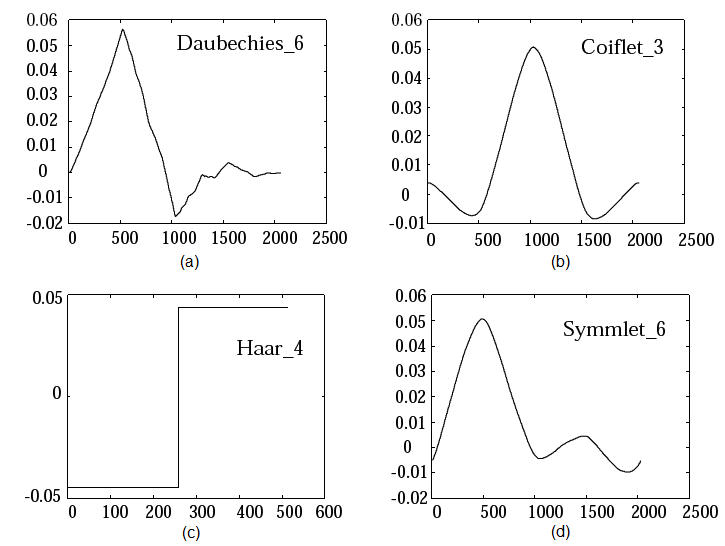
\includegraphics[width=3in]{img/waveletContinuaFamilias}
	\caption{Famílias de TWC: (a) Daubechies; (b) Coiflet; (c) Haar; (d) Symmlet.}
	\label{waveletContinuaFamilias}
\end{figure}

A Transformada \textit{Wavelet} Discreta (TWD) permite não perder suas qualidades e propriedades, portando-se de maneira numericamente estável e com uma menor redundância de informação \cite{silva06}. A sua realização acontece por meio de filtragens digitais sucessivas sobre o sinal
original, onde um par de filtros digitais definidos como filtros em quadratura é descrito pelas funções h(n) e g(n), sendo estas, respectivamente, as funções resposta ao impulso de um filtro passa-baixa e passa-alta, cada um com metade da banda do sinal original \cite{castelano06}. Ela é matematicamente definida em $F_{m,n}(a,b)$:

\[ 	F_{m,n}(a,b) = a_{0}^{-j/2}\int f(t)\Psi (a_{0}^{-j}t - nb_{0}) \]

\subsection{Classificação de Sinais}
Como o objetivo do trabalho consiste na análise e classificação de arritmias por meio de Aprendizado de Máquina, faz-se necessário realizar a extração das características dos sinais para poder classificar com um certo grau de confiabilidade por meio de algum algoritmo de inteligência artificial.

O primeiro passo necessário para a classificação de sinais se encontra na normalização do sinal de ECG afim de obter e tratar pedaços de amostras obtidas do sinal. Para realizar esse processo utilizam-se diversos tipos de funções matemáticas, selecionando as amostras filtradas - por janelamento e DWT com extração dos coeficientes, por exemplo - ou através de extração de características diretas do sinal, como o intervalo RR e frequência cardíaca.

\subsection{Aprendizado de Máquina}

O aprendizado de máquina se caracteriza por ser um subcampo dentro de toda a inteligência artificial, e tem o objetivo de desenvolver algoritmos e técnicas que permitam os computadores adquirirem conhecimento sem serem explicitamente programados. Dado um conjunto de amostras cujo tenha classificação conhecida, a máquina conseguem interpretar os dados e classificá-los, aprendendo com seus erros \cite{morellato08}. As técnicas do aprendizado de máquina podem ser aplicadas em diversas áreas do conhecimento, como em problemas relacionados a computação, biologia, química e matemática \cite{morellato08}.

Os algoritmos de aprendizados de máquinas podem ser divididos em dois principais tipos: os supervisionados e não supervisionados. O aprendizado de máquina supervisionado trata de amostras no qual foram fornecidas uma referência do objetivo, disponibilizando para o computador informações a respeito do ambiente em que as amostras pertencem \cite{marr2017}. Neste tipo de aprendizado, em cada amostra é fornecida variáveis de entrada e a saída esperada, também chamada de \textit{true label}. Ao final do treinamento, é esperado que a máquina seja capaz de fornecer saídas corretas para entradas que nunca foram apresentadas. O aprendizado de máquina não supervisionado não contém o \textit{true label}, tendo amostras compostas apenas pelas variáveis de entrada.Com isso, os algoritmos não supervisionadas tentam encontrar padrões nas amostras fornecidas, separando-as em grupos \cite{marr2017}.


O cérebro em alguns aspectos possui características similares a um processador. Por exemplo, quando lemos um texto as células fotorreceptoras dos nossos olhos captam um conjunto de símbolos e os transformam em sinais elétricos, que por sua vez, serão processados pelo cérebro para classificá-los em palavras. As redes neurais artificiais (RNAs) consistem em uma metodologia para resolver problemas de inteligência artificial que se espelham em conceitos das rede neurais naturais (RNN). O comportamento de aprendizagem da RNA é igual ao da RNN, ou seja, aprendendo, errando e fazendo descobertas. As unidades de processamento são chamadas neurônios, que são compostos basicamente por dendritos, axônio e corpo celular \cite{kovacs96}. A relação entre um neurônio natural e um \textit{Perceptron} ou neurônio booleano foi representada pela Tabela \ref{table:tabelaComparativaNeuronioPerceptron}.

\renewcommand\tablename{TABELA}
\begin{table}[!h]
	%% increase table row spacing, adjust to taste
	\renewcommand{\arraystretch}{1.3}
	% if using array.sty, it might be a good idea to tweak the value of
	% \extrarowheight as needed to properly center the text within the cells
	\caption{Relação entre um neurônio natural e um \textit{Perceptron}}
	\label{table:tabelaComparativaNeuronioPerceptron}
	\centering
	%% Some packages, such as MDW tools, offer better commands for making tables
	%% than the plain LaTeX2e tabular which is used here.
	\begin{tabular}{|c|c|c|}
		\hline
		\textbf{\textit{Perceptron}} & \textbf{Neurônio Natural} & \textbf{Função}\\
		\hline
		Entradas & Dendritos & Recebem o sinal \\		
		\hline
		Saída & Axônio & Saída do sinal \\		
		\hline
		Peso & Sinapse & Retém o Conhecimento \\		
		\hline
	\end{tabular}
\end{table}

 
Para classificar o sinal normalizado serão utilizados os algoritmos: \textit{Random Forest} e \textit{Artificial Neural Networks}.

O algoritmo \textit{Random Forest} consiste na criação aleatória de um conjunto de árvores simples de decisão, em que cada uma delas produz uma resposta, dado um conjunto de valores apresentados previamente \cite{statsoft09}. Para a classificação de um resultado final, é verificado os resultados independentes de cada árvore gerada, realizando uma votação, em que é elegido o resultado mais votado. A classificação de cada árvore se encontra nos nós folhas de cada árvore criada \cite{dantas2015}.

O algoritmo de Redes Neurais Artificiais, por sua vez, pode ser definido como técnicas computacionais que apresentam uma estrutura inspirada nas redes neurais de organismos inteligentes, que aprendem a partir de experiências \cite{carvalho09}. A estrutura de uma rede neural artificial é composta por unidades interconectadas, que representam os neurônios, em que cada um tem determinado comportamento baseado em suas entradas \cite{zuben03}. Cada neurônio artificial tem entradas que são saídas de outros neurônios. Cada entrada é multiplicada por um peso específico, sendo que esse peso indica sua influência para a saída daquela unidade. Com todos os valores de entradas calculados, é realizada uma soma ponderada, e o valor dessa soma é inserido em uma função para a normalização, gerando o valor de saída daquele neurônio. Chegando ao final da rede neural artificial, é feito o caminho contrário para atualizar os pesos das ligações de cada unidade, também chamado de \textit{backpropagation} \cite{zuben03}. O ciclo de calcular um resultado e atualizar os pesos é denominado como uma época,sendo que para  um treinamento de uma rede neural artificial é necessário várias épocas \cite{carvalho09}.

% An example of a floating figure using the graphicx package.
% Note that \label must occur AFTER (or within) \caption.
% For figures, \caption should occur after the \includegraphics.
% Note that IEEEtran v1.7 and later has special internal code that
% is designed to preserve the operation of \label within \caption
% even when the captionsoff option is in effect. However, because
% of issues like this, it may be the safest practice to put all your
% \label just after \caption rather than within \caption{}.
%
% Reminder: the "draftcls" or "draftclsnofoot", not "draft", class
% option should be used if it is desired that the figures are to be
% displayed while in draft mode.
%
%\begin{figure}[!b]
%\centering
%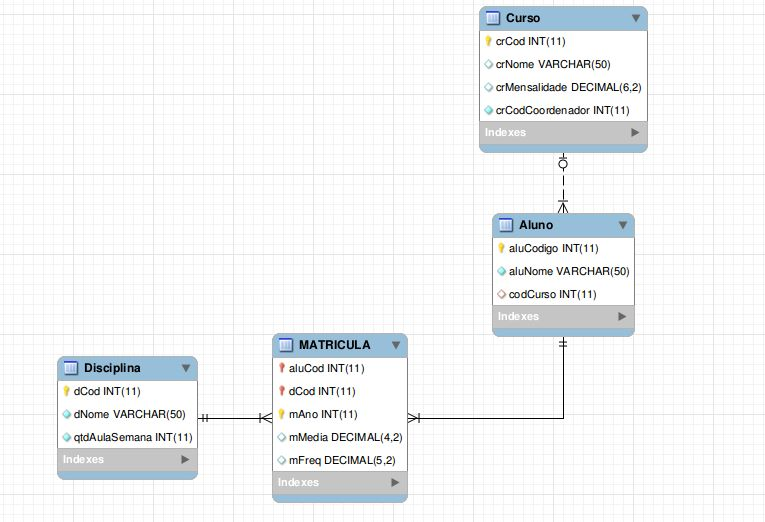
\includegraphics[width=2.5in]{myfigure}
% where an .eps filename suffix will be assumed under latex, 
% and a .pdf suffix will be assumed for pdflatex; or what has been declared
% via \DeclareGraphicsExtensions.
%\caption{Simulation results for the network.}
%\label{fig_sim}
%\end{figure}

% Note that the IEEE typically puts floats only at the top, even when this
% results in a large percentage of a column being occupied by floats.


% An example of a double column floating figure using two subfigures.
% (The subfig.sty package must be loaded for this to work.)
% The subfigure \label commands are set within each subfloat command,
% and the \label for the overall figure must come after \caption.
% \hfil is used as a separator to get equal spacing.
% Watch out that the combined width of all the subfigures on a 
% line do not exceed the text width or a line break will occur.
%
%\begin{figure*}[!b]
%\centering
%\subfloat[Case I]{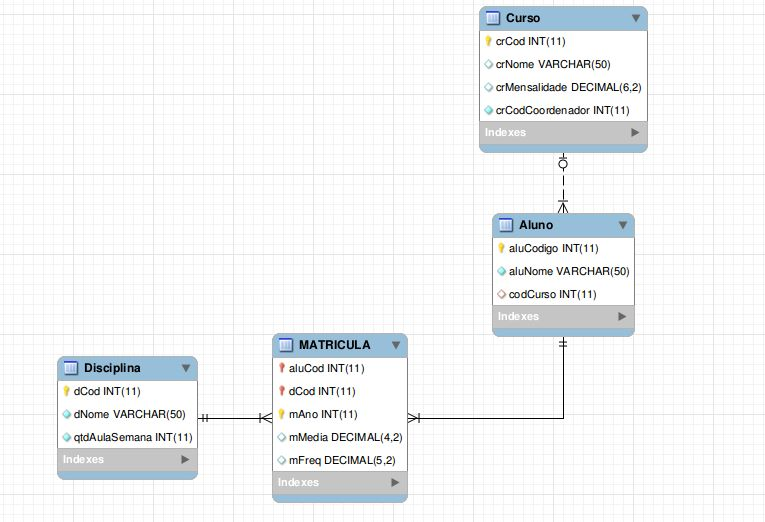
\includegraphics[width=2.5in]{box}%
%\label{fig_first_case}}
%\hfil
%\subfloat[Case II]{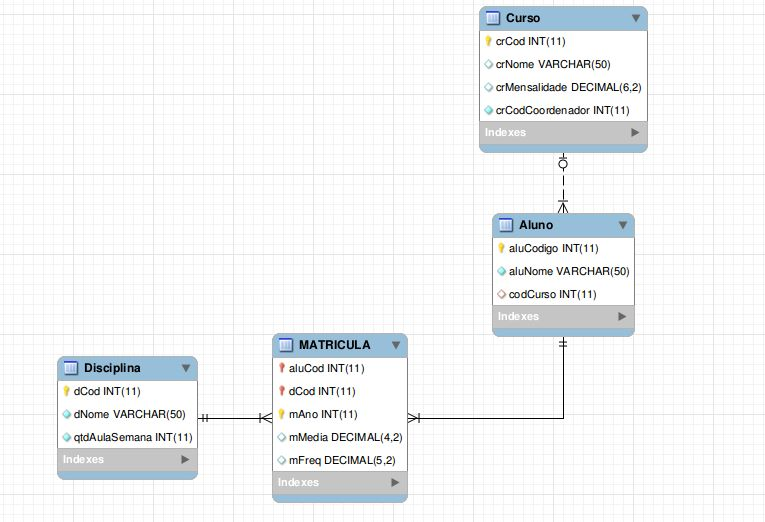
\includegraphics[width=2.5in]{box}%
%\label{fig_second_case}}
%\caption{Simulation results for the network.}
%\label{fig_sim}
%\end{figure*}
%
% Note that often IEEE papers with subfigures do not employ subfigure
% captions (using the optional argument to \subfloat[]), but instead will
% reference/describe all of them (a), (b), etc., within the main caption.
% Be aware that for subfig.sty to generate the (a), (b), etc., subfigure
% labels, the optional argument to \subfloat must be present. If a
% subcaption is not desired, just leave its contents blank,
% e.g., \subfloat[].


% Note that the IEEE does not put floats in the very first column
% - or typically anywhere on the first page for that matter. Also,
% in-text middle ("here") positioning is typically not used, but it
% is allowed and encouraged for Computer Society conferences (but
% not Computer Society journals). Most IEEE journals/conferences use
% top floats exclusively. 
% Note that, LaTeX2e, unlike IEEE journals/conferences, places
% footnotes above bottom floats. This can be corrected via the
% \fnbelowfloat command of the stfloats package.


\section{Metodologia}

A partir da proposta e fundamentação teórica apresentada, pode-se determinar quais ferramentas utilizadas e qual metodologia empregada no projeto. 

O projeto foi desenvolvido em duas etapas: primeiro o tratamento do sinal para extração de características, e depois o treinamento das arritmias por aprendizado de máquina.

O objetivo do tratamento do sinal foi isolar partes do sinal do ECG por janelamento para, consequentemente, conseguir aplicar \textit{Transformadas Wavelets Discretas} para filtro e redução de ruídos. Através do \textit{software MATLAB}, o janelamento de períodos do sinal foi realizado através de arquivos de anotações da base de dados de arritmia, as quais possuíam exatos períodos de tempo onde a arritmia a ser verificada ocorria.

A partir do sinal normalizado e tratado, realizou-se a extração de duas características cardíacas importantes para posterior treinamento: amplitude da onda R em milivolts (mV) e intervalo de tempo entre ondas R em segundos (seg). Esses dados foram extraídos em arquivos do tipo CSV juntamente com um \textit{true label}, variável a qual caracteriza o tipo de arritmia.

Por fim, com os arquivos contendo as características extraídas dos sinais normalizados, foi possível realizar o aprendizado de máquina com o \textit{software WEKA}. Para fim de validação de qual método seria mais eficaz, foi realizado uma comparação entre o treinamento com um algoritmo de Redes Neurais e outro de Árvores de Decisão, utilizando 80\% da base de dados como treinamento e 20\% como teste.

Todo o código desenvolvido e resultados obtidos apresentados nesse trabalho podem ser acessados através do repositório aberto utilizado no \textit{Github} \cite{kawasaki17}.

% An example of a floating table. Note that, for IEEE style tables, the
% \caption command should come BEFORE the table and, given that table
% captions serve much like titles, are usually capitalized except for words
% such as a, an, and, as, at, but, by, for, in, nor, of, on, or, the, to
% and up, which are usually not capitalized unless they are the first or
% last word of the caption. Table text will default to \footnotesize as
% the IEEE normally uses this smaller font for tables.
% The \label must come after \caption as always.
%

%\renewcommand\tablename{TABELA}
%\begin{table}[!h]
%% increase table row spacing, adjust to taste
%\renewcommand{\arraystretch}{1.3}
% if using array.sty, it might be a good idea to tweak the value of
% \extrarowheight as needed to properly center the text within the cells
%\caption{Cronograma de Tópicos Trabalhados do Projeto}
%\label{table:cronogramaProjeto}
%\centering
%% Some packages, such as MDW tools, offer better commands for making tables
%% than the plain LaTeX2e tabular which is used here.
%\begin{tabular}{|c|c|}
%\hline
%Semana 01/05 & Estudo do contexto do artigo\\
%\hline
%Semana 08/05 & Estudo de ECG e extração dos dados\\
%\hline
%Semana 15/05 & Estudo de transformada \textit{Wavelet}\\
%\hline
%Semana 22/05 & Estudo da aplicação de Redes Neurais e Algoritmos\\
%\hline
%Semana 29/05 & Extração e Classificação dos Sinais com \textit{Wavelet}\\
%\hline
%Semana 05/06 & Execução dos Aprendizados Supervisionados\\
%\hline
%Semana 12/06 & Análise dos Aprendizados e Geração do Relatório\\
%\hline
%Semana 19/06 & Finalização do Relatório e Apresentação Final\\
%\hline
%\end{tabular}
%\end{table}

\section{Extração de Características}

Conforme apresentado no tópico anterior, a normalização de sinal e extração de características foram realizadas através do \textit{software MATLAB}. Essa etapa foi fundamental para que fosse elaborado um algoritmo modular e completo, capaz de realizar desde o janelamento do sinal até a extração das características para o treinamento com aprendizado de máquina, o qual será detalhado no próximo tópico.

Para uma melhor compreensão desse algoritmo, é necessário compreender o funcionamento da base de dados de arritmia do MIT-BIH. A base conta com 48 amostras de diferentes pessoas, sendo que cada uma das amostras possui uma duração de aproximadamente 30 minutos e com janelas aleatórias de diferentes tipos de arritmias. Para cada amostra é possível realizar a extração de vários tipos de arquivos, onde nesse trabalho três tipos foram focados: extração do sinal com uma faixa (potencial MLII, derivado do tipo V2) em um arquivo .mat, extração de informações do sinal completo em um arquivo .info e, por fim, extração de detalhes de cada período de sinal com os tipos de arritmias - provenientes de considerações de profissionais cardiologistas - em um arquivo .txt. Um exemplo do arquivo de anotações pode ser visualizado através da Figura \ref{ecgSignalAnnotationsExample}, onde é possível visualizar um tipo de arritmia do tipo Bigeminismo (B no período 0:00.186 ou na amostra 67 do sinal.

\begin{figure}[!h]
	\centering
	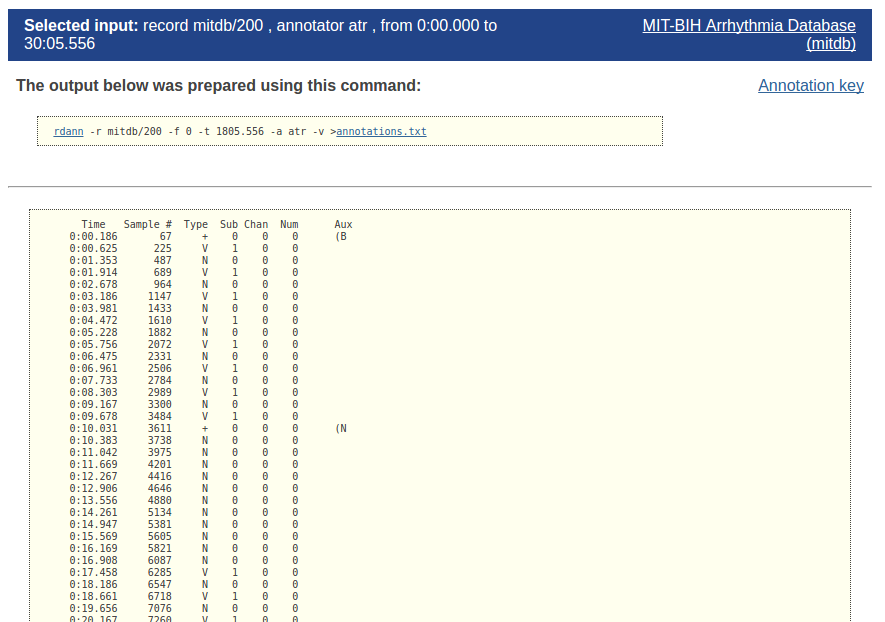
\includegraphics[width=3in]{img/ecgSignalAnnotationsExample}
	\caption{Exemplo de anotações extraídas do sinal ECG 100m dentro do site da Physionet ATM.}
	\label{ecgSignalAnnotationsExample}
\end{figure}

Com os 3 arquivos de 17 amostras de sinais foi possível realizar a normalização e extração das 3 arritmias propostas através de 6 etapas realizadas no \textit{MATLAB} para cada uma das 17 amostras:

1. A primeira etapa consistiu em carregar cada um dos 17 sinais de ECG, extraindo os valores elétricos em amplitude e tempo, além da frequência, quantidade de amostras e tempo total do sinal.

2. Em seguida, realizou-se a leitura do arquivo de anotações dos sinais, capturando em um objeto de vetores os períodos e tempos das amostras da arritmia escolhida para extração.

3. Com cada um dos períodos específicos das arritmias, foi possível realizar o janelamento da parte QRS de cada onda, capturando um intervalo de tempo anterior e posterior a amostra de tempo da arritmia extraída na etapa anterior. 

4. Após a extração do sinal em amplitude e tempo em um objeto de vetores do janelamento, realiza-se a plotagem de cada sinal QRS extraído, exceto para casos sem arritmia - chamados de \textit{Normal Sinus Rhythm (N)}. Uma extração do janelamento da parte QRS do arquivo 201m pode ser visualizada na Figura \ref{signalQRSExtractedTrigeminy}, onde foi extraída arritmia Trigeminismo Ventricular.

\begin{figure}[!h]
	\centering
	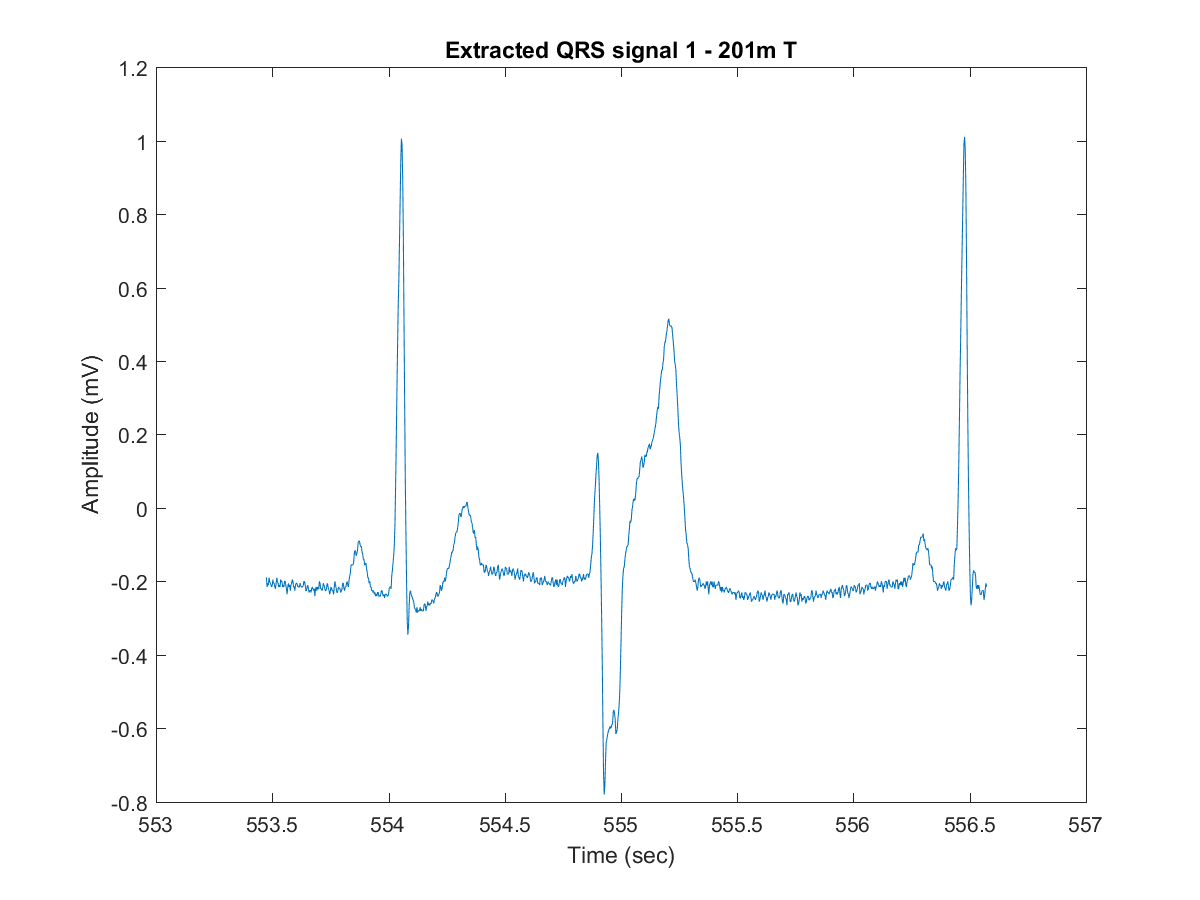
\includegraphics[width=3in]{img/signalQRSExtractedTrigeminy}
	\caption{Sinal QRS de Trigeminismo Ventricular extraído por janelamento do arquivo 201m.}
	\label{signalQRSExtractedTrigeminy}
\end{figure}

5. Com as janelas dos sinais separados em objeto de vetores realiza-se a decomposição de cada sinal janelado em componentes de frequência variantes no tempo com Transformada \textit{Wavelet} Discreta de Sobreposição Máxima (MODWT) e Transformada \textit{Wavelet} Discreta Inversa de Sobreposição Máxima (IMODWT) na escala 3 - funções disponíveis através do \textit{Wavelet Toolbox} do \textit{software MATLAB}.

5. Após a extração do sinal modulado e filtrado com \textit{Transformada Wavelet Discreta}, realizou-se a extração da amplitude e tempo dos picos do sinal janelado através da função \textbf{findpeaks} do \textit{Signal Processing Toolbox}.

6. Após a extração dos picos em um objeto de vetores, realiza-se a plotagem de cada sinal com seus respectivos pontos de pico, exceto para casos sem arritmia (N). Uma extração do picos do arquivo 201m pode ser visualizada na Figura \ref{signalPeaksExtractedTrigeminy}, onde foi extraída arritmia Trigeminismo Ventricular.

\begin{figure}[!h]
	\centering
	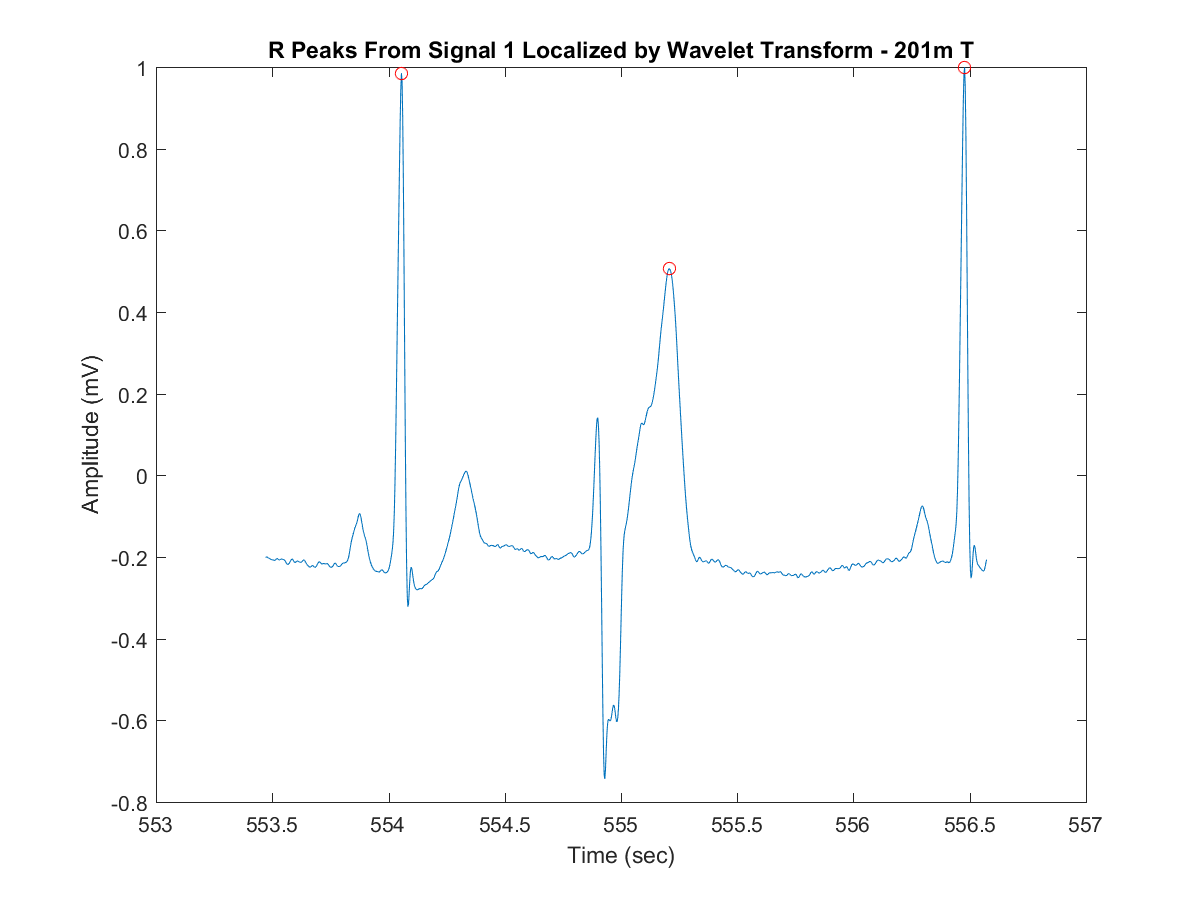
\includegraphics[width=3in]{img/signalPeaksExtractedTrigeminy}
	\caption{Picos de Trigeminismo Ventricular extraídos do arquivo 201m.}
	\label{signalPeaksExtractedTrigeminy}
\end{figure}

7. Por fim, com os dados de amplitude e tempo extraídos em um objeto de vetores, realizou-se a extração de características, capturando o valor de amplitude do último pico do sinal e a diferença de tempo R-R entre o último e o primeiro pico (o pico do meio não se caracteriza como pico R). Após a manipulação desses dados, realiza-se a extração dessas duas características com o tipo da arritmia em um arquivo CSV, populando cada linha do arquivo com cada período de amostra encontrado para a arritmia escolhida. Um arquivo CSV extraído para o Trigeminismo Ventricular pode ser visualizado na Figura \ref{trigeminyFeaturesExtractedCSVExample}.

\begin{figure}[!h]
	\centering
	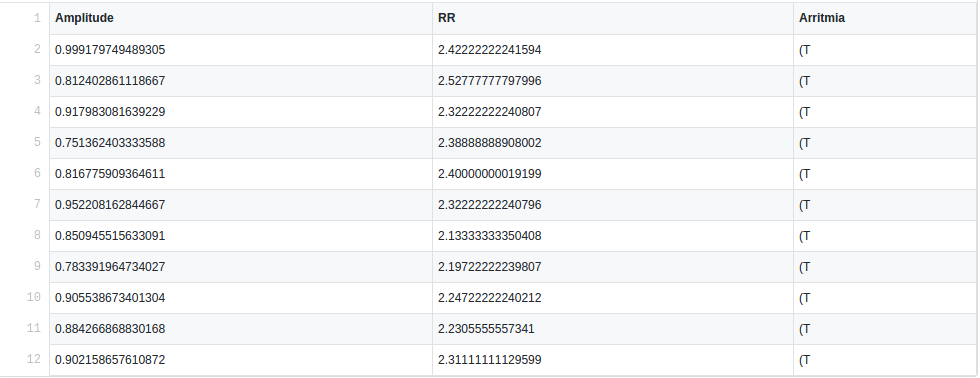
\includegraphics[width=3in]{img/trigeminyFeaturesExtractedCSVExample}
	\caption{Arquivo de características extraído para Trigeminismo Ventricular referentes ao arquivo 201m.}
	\label{trigeminyFeaturesExtractedCSVExample}
\end{figure}

Essas etapas apresentadas foram executadas para cada um dos 17 arquivos e para todas as arritmias, além do arquivo 100m para extração de características de um sinal saudável (N). Após a extração de todos os CSVs, organizou-se em um só arquivo com todas as características de todos tipos de arritmias, o qual foi repassado para ser inserido no aprendizado de máquina.

\section{Treinamento com Aprendizado de Máquina}

\textbf{Aqui vai a parte do Weka.}

\begin{figure}[!h]
	\centering
	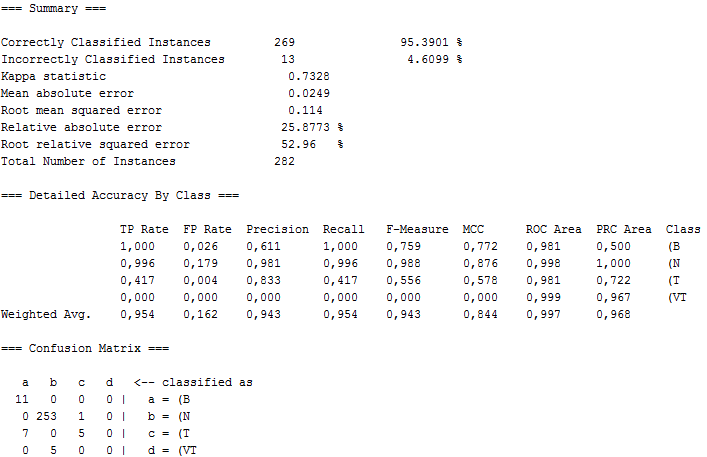
\includegraphics[width=3in]{img/wekaResultANN8020}
	\caption{Resultados do treinamento com Redes Neurais no \textit{software WEKA}.}
	\label{wekaResultANN8020}
\end{figure}

\begin{figure}[!h]
	\centering
	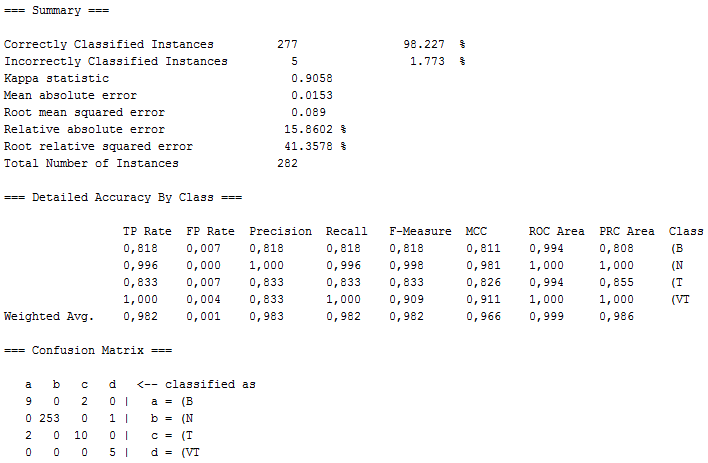
\includegraphics[width=3in]{img/wekaResultRandomForest8020}
	\caption{Resultados do treinamento com Árvores de Decisão no \textit{software WEKA}.}
	\label{wekaResultRandomForest8020}
\end{figure}

\section{Resultados e Discussões}

A partir dos resultados obtidos com o aprendizado de máquina, foi possível analisar a eficiência do método de extração de características e dos algoritmos de aprendizado na área de ECG.

Conforme pode ser visualizado nos resultados do treinamento com Redes Neurais - representado pela Figura \ref{wekaResultANN8020} - a arritmia do tipo Bigeminismo Ventricular e os casos normais (sem arritmia) foram classificadas com eficiência nos testes, enquanto as arritmias do tipo Trigeminismo e Taquicardia Ventricular não foram classificadas adequadamente. Com esses resultados, algumas considerações podem ser feitas: o método de normalização e extração de características pelo \textit{software MATLAB} foi extremamente eficiente no caso do Bigeminismo e do tipo Normal, demonstrando que precisa ser aprimorado para extração das características dos outros dois tipos de arritmia; a outra consideração pode estar presente na quantidade de características extraídas, as quais podem não ter sido suficientes para classificação dos tipos Trigeminismo e Taquicardia Ventricular.

Em contraposição, os resultados do treinamento com Árvores de Decisão - representado pela Figura \ref{wekaResultRandomForest8020} - demonstram um treinamento e teste eficiente, com classificação correta de cada tipo de arritmia, onde os casos de Bigeminismo e Trigeminismo Ventricular apresentam apenas duas classificações erradas nos testes.

A partir dos resultados de acurácia apresentados através da Tabela \ref{table:tabelaResultadosAprendizadoMaquina}, foi possível verificar que, com as características extraídas para testes de ECG, o aprendizado de máquina utilizando o algoritmo de Árvores de Decisão \textit{Random Forest} apresentou-se como mais adequado para utilização, com pior caso para Bigeminismo com 81,8\%. Os resultados apresentados provavelmente poderiam ser melhores se fossem realizados com uma maior quantidade de amostras tanto para treinamento quanto para teste.

\renewcommand\tablename{TABELA}
\begin{table}[!h]
	%% increase table row spacing, adjust to taste
	\renewcommand{\arraystretch}{1.3}
	% if using array.sty, it might be a good idea to tweak the value of
	% \extrarowheight as needed to properly center the text within the cells
	\caption{Resultados de Acurácia para Aprendizado de Máquina utilizando Rede Neural e Árvores de Decisão}
	\label{table:tabelaResultadosAprendizadoMaquina}
	\centering
	%% Some packages, such as MDW tools, offer better commands for making tables
	%% than the plain LaTeX2e tabular which is used here.
	\begin{tabular}{|c|c|c|}
		\hline
		\textbf{Tipo de Arritmia} & \textbf{Redes Neurais} & \textbf{\textit{Random Forest}}\\
		\hline
		(B & 100\% & 81,8\% \\		
		\hline
		(N & 99,6\% & 99,6\% \\		
		\hline
		(T & 41,7\% & 83,3\% \\		
		\hline
		(VT & 0\% & 100\% \\		
		\hline
	\end{tabular}
\end{table}

\section{Conclusão}

O tratamento de pacientes tem sido uma preocupação global, onde cada vez mais pessoas precisam ser diagnosticadas por uma porcentagem pequena de médicos extremamente ocupados. Sendo assim, métodos automáticos de diagnósticos têm sido desenvolvidos para auxiliar profissionais da saúde, principalmente em áreas que ainda não foram totalmente "convertidas" para o meio digital.

Nesse contexto, uma das áreas que tem evoluído com vários trabalhos e artigos consiste em exames cardiológicos \cite{beckert09}  \cite{barrella14} \cite{manzan06}, que normalmente são manuais e ainda analógicos, dependentes da avaliação final de um profissional médico.

O objetivo desse trabalho, portanto, foi contribuir no diagnóstico automático e digital de arritmias em um exame de ECG, auxiliando o processo decisório de um profissional de cardiologia. Por meio da extração de características cardíacas de sinais específicos, foi possível realizar um aprendizado de máquina, conseguindo treinar uma inteligência artificial para identificação de três arritmias baseado nas características disponibilizadas.

Conforme apresentado no tópico anterior, a extração e treinamento conseguiram apresentar resultados satisfatórios, principalmente para o algoritmo de treinamento \textit{Random Forest}. O trabalho, portanto, apresentou uma alternativa rápida e inicial para um diagnóstico cardíaco. Contudo, alguns pontos podem ter comprometido o trabalho, e podem contribuir para trabalhos futuros:

1. A falta de quantidade de amostras de arritmias pode ter influenciado no resultado, dado que a grande maioria das amostras eram do tipo Normal (254 na parte de teste, por exemplo). A base de dados de arritmias do MIT-BIH pode ser aprimorada, contendo uma maior quantidade de sinais com mais ocasiões de arritmias.

2. A estratégia de extração do complexo QRS por janelamento pode ter comprometido a qualidade da acurácia do treinamento, dado que nesse trabalho não foram identificados os diferentes tipos de onda de um batimento de ECG. Ou seja, para trabalhos futuros uma extração das ondas P, QRS, T podem melhorar a qualidade do trabalho, assim como conseguir identificar outros tipos de arritmias - como o caso da Fibrilação Atrial, que ocorre na despolarização atrial da onda P.

3. A estratégia de coleta dos picos precisa ser aprimorada, dado que cada tipo de arritmia pode caracterizar uma quantidade de picos diferentes, ou até picos falsos que podem comprometer a extração adequada para treinamento.

4. A quantidade de características cardíacas extraídas para treinamento também pode ter influenciado o resultado, dado que aprendizado de máquina possui uma maior eficiência com uma grande quantidade de amostras e características relevantes ao estudo empregado. Sendo assim, um possível aprimoramento poderia ser a extração de outras características, como: amplitude mínima da onda R, média e raiz quadrada da amplitude, derivada máxima da amplitude e seu período (captura a velocidade da onda R), e derivada absoluta média \cite{barrella14}.

Por fim, esse trabalho foi importante para contribuir ainda mais com o conhecimento médico digital, oferecendo uma solução alternativa para uma evolução de diagnósticos cardiológicos.

% conference papers do not normally have an appendix


% use section* for acknowledgment
\section*{Agradecimentos}

Os autores gostariam de agradecer o prof. Danilo Hernane Spatti pela supervisão e orientação na elaboração desse projeto.

% trigger a \newpage just before the given reference
% number - used to balance the columns on the last page
% adjust value as needed - may need to be readjusted if
% the document is modified later
%\IEEEtriggeratref{8}
% The "triggered" command can be changed if desired:
%\IEEEtriggercmd{\enlargethispage{-5in}}

% references section

% can use a bibliography generated by BibTeX as a .bbl file
% BibTeX documentation can be easily obtained at:
% http://mirror.ctan.org/biblio/bibtex/contrib/doc/
% The IEEEtran BibTeX style support page is at:
% http://www.michaelshell.org/tex/ieeetran/bibtex/
\def\refname{Referências}
\bibliographystyle{IEEEtran}
% argument is your BibTeX string definitions and bibliography database(s)
\bibliography{IEEEabrv}
%
% <OR> manually copy in the resultant .bbl file
% set second argument of \begin to the number of references
% (used to reserve space for the reference number labels box)
%\begin{thebibliography}{1}

%\bibitem{IEEEhowto:kopka}
%H.~Kopka and P.~W. Daly, \emph{A Guide to \LaTeX}, 3rd~ed.\hskip 1em plus
%  0.5em minus 0.4em\relax Harlow, England: Addison-Wesley, 1999.

% \end{thebibliography}




% that's all folks
\end{document}


